% $ platex body
% $ dvipdfmx body

\documentclass[a4j]{jarticle}

\title{「西洋音楽の歴史と理論」報告課題}
\author{KR17074 山内 拓弥}
\date{平成29年9月xx日}
\usepackage{colortbl}
\usepackage[dvipdfmx]{graphicx}
%\renewcommand{\thesection}{課題\arabic{section}}
%\renewcommand{\thesubsection}{}

\begin{document}

%\maketitle

\section{教皇の権威の低下とルネサンス}

\begin{table}[tb]
 \begin{center}
  \caption{西ヨーロッパ中世とルネサンスの比較}
  \label{tab:comparison}
  \begin{tabular}{|l|l|} \hline
  中世                       & ルネサンス                         \\
  \hline \hline
  教皇が絶大な権力を持つ。   & 教皇の権威が低下、国王が力を持つ。 \\ \hline
  神が中心。                 & 人間が中心。                       \\ \hline
  地球は平坦、天動説。       & 地球は球形、地動説。               \\ \hline
  和音は、神学的理論を優先。 & 和音は、人間の聴覚を優先。         \\
  5度音程が中心。            & 3度、6度のやわらかい響きを多用。   \\ \hline
  \end{tabular}
 \end{center}
\end{table}

\section{ルネサンスの音楽}

\begin{figure}[tb]
 \begin{center}
  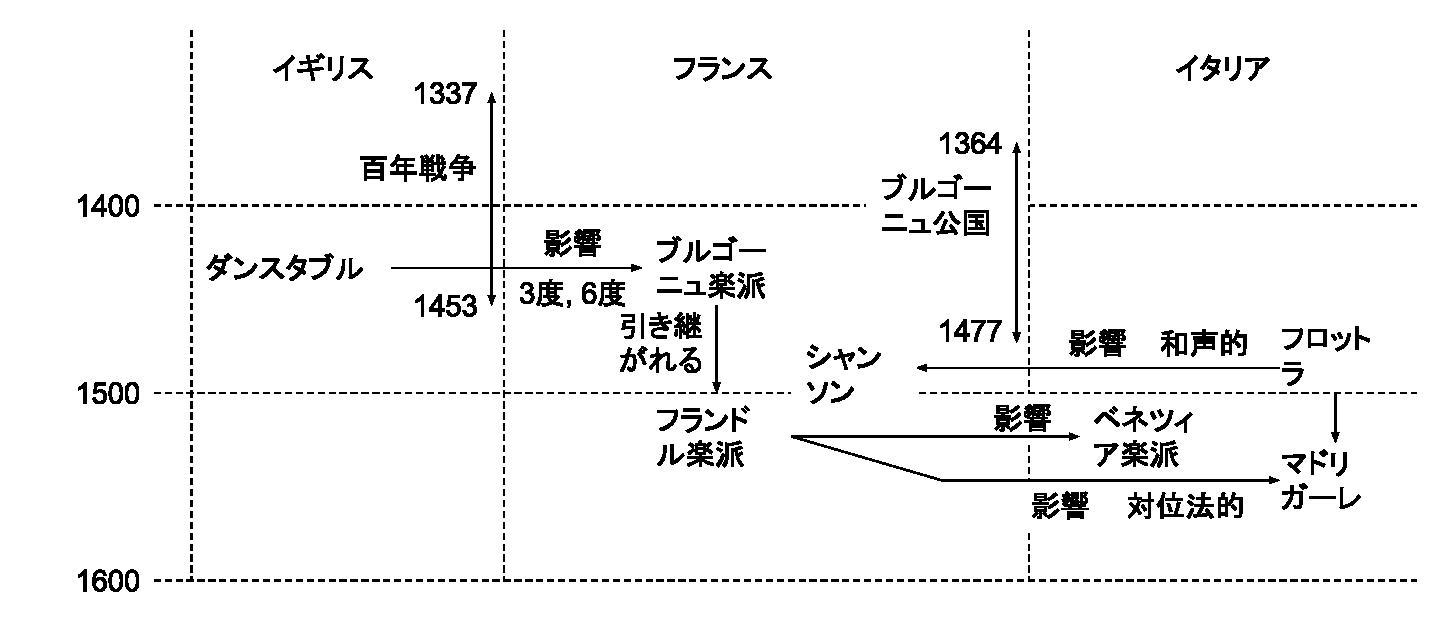
\includegraphics[width=\hsize]{fig/renaissance_summary.eps}
  \caption{ルネサンス音楽概略}
  \label{fig:renaissance_summary}
 \end{center}
\end{figure}

\end{document}
